%%%%%%%%%%%%%%%%%%%%%%%%%%%%%%%%%%%%%%%%%%%%%%%%%%%%%%%%%%%%%%%%%%%%%%%%%%%%%%%%%%
\begin{frame}[fragile]\frametitle{}
\begin{center}
{\Large Deep Learning for NLP with Pytorch (0.4.0)}

(Ref:  Robert Guthrie -  https://pytorch.org/tutorials/beginner/deep\_learning\_nlp\_tutorial.html)
\end{center}
\end{frame}



%%%%%%%%%%%%%%%%%%%%%%%%%%%%%%%%%%%%%%%%%%%%%%%%%%%%%%%%%%%%%%%%%%%%%%%%%%%%%%%%%%
\begin{frame}[fragile]
\frametitle{Logistic Regression Bag-of-Words classifier}

\begin{itemize}
\item Input: a sparse bag-of-words representation
\item Output: probability distribution over two labels: ``English'' and ``Spanish''. 
\item Model: Logistic regression.
\end{itemize}
 \begin{lstlisting}
data = [(''me gusta comer en la cafeteria''.split(), ''SPANISH''),
        (''Give it to me''.split(), ''ENGLISH''),
        (''No creo que sea una buena idea''.split(), ''SPANISH''),
        (''No it is not a good idea to get lost at sea''.split(), ''ENGLISH'')]

test_data = [(''Yo creo que si''.split(), ''SPANISH''),
             (''it is lost on me''.split(), ''ENGLISH'')]
\end{lstlisting}              
\end{frame} 



%%%%%%%%%%%%%%%%%%%%%%%%%%%%%%%%%%%%%%%%%%%%%%%%%%%%%%%%%%%%%%%%%%%%%%%%%%%%%%%%%%
\begin{frame}[fragile]
\frametitle{BoW}

\begin{itemize}
\item Assign each word in the vocab an index. For example, say our entire vocab is two words ''hello'' and ''world'', with indices 0 and 1 respectively.
\item The BoW vector for the sentence ''hello hello hello hello'' is $$ \left[ 4, 0 \right] $$ For ''hello world world hello'', it is $$ \left[ 2, 2 \right] $$ etc.
\item In general, it is  $$ \left[ \text{Count}(\text{hello}), \text{Count}(\text{world}) \right] $$
\end{itemize}
 \begin{lstlisting}
word_to_ix = {}
for sent, _ in data + test_data:
    for word in sent:
        if word not in word_to_ix:
            word_to_ix[word] = len(word_to_ix)
print(word_to_ix)
>>>{'is': 16, 'lost': 21, 'creo': 10, 'Give': 6, 'Yo': 23, 'me': 0, 'to': 8, 'good': 19, 'at': 22, 'it': 7, 'a': 18, 'comer': 2, 'not': 17, 'get': 20, 'si': 24, 'cafeteria': 5, 'gusta': 1, 'sea': 12, 'buena': 14, 'la': 4, 'una': 13, 'on': 25, 'idea': 15, 'No': 9, 'que': 11, 'en': 3}

label_to_ix = {''SPANISH'': 0, ''ENGLISH'': 1}
\end{lstlisting}              
\end{frame} 


%%%%%%%%%%%%%%%%%%%%%%%%%%%%%%%%%%%%%%%%%%%%%%%%%%%%%%%%%%%%%%%%%%%%%%%%%%%%%%%%%%
\begin{frame}[fragile]
\frametitle{NN}

\begin{itemize}
\item Inheriting from nn.Module!
\item Init here calls the init function of nn.Module. (should do it always!!)
\item Define the parameters that you will need: Weights and Biases
\item Weights will have size of the vocab.
\item Output is same as num labels (2)
\item Forward method defines Actications taking inputs in vector form, thats it.
\end{itemize}
 \begin{lstlisting}
class BoWClassifier(nn.Module): 
    
    def __init__(self, num_labels, vocab_size):
    		super(BoWClassifier, self).__init__()
    		self.linear = nn.Linear(vocab_size, num_labels)

	def forward(self, bow_vec):
		return F.log_softmax(self.linear(bow_vec))
    
\end{lstlisting}              
\end{frame} 

%%%%%%%%%%%%%%%%%%%%%%%%%%%%%%%%%%%%%%%%%%%%%%%%%%%%%%%%%%%%%%%%%%%%%%%%%%%%%%%%%%
\begin{frame}[fragile]
\frametitle{Preparing Input}

\begin{itemize}
\item Take a sentance and make a Bow Vector of it.
\item Allocate for full vocab length, and go on increementinfg indeices of all words in the sentence
\item For lables, make similar one hot encoding
\end{itemize}
 \begin{lstlisting}
def make_bow_vector(sentence, word_to_ix):
    vec = torch.zeros(len(word_to_ix))
    for word in sentence:
        vec[word_to_ix[word]] += 1
    return vec.view(1, -1)

def make_target(label, label_to_ix):
    return torch.LongTensor([label_to_ix[label]])
\end{lstlisting}              
\end{frame} 


%%%%%%%%%%%%%%%%%%%%%%%%%%%%%%%%%%%%%%%%%%%%%%%%%%%%%%%%%%%%%%%%%%%%%%%%%%%%%%%%%%
\begin{frame}[fragile]
\frametitle{Model}

\begin{itemize}
\item Instantiate the model
\item It initializes all the weights.
\end{itemize}
 \begin{lstlisting}
VOCAB_SIZE = len(word_to_ix)
NUM_LABELS = 2 
model = BoWClassifier(NUM_LABELS, VOCAB_SIZE)

for param in model.parameters():
    print(param)
    
>>>Parameter containing:
tensor([[-0.1001, -0.1382, -0.1625,  0.1922, -0.0334, -0.0453, -0.0721,
         -0.0981, -0.1794, -0.1151,  0.1199,  0.0430, -0.0692, -0.0741,
          0.1253,  0.1414,  0.1889,  0.0572,  0.0947, -0.0158, -0.1147,
         -0.1921,  0.1195, -0.0285,  0.0806,  0.0097],
        [-0.1830, -0.0962,  0.0552, -0.0397, -0.1894,  0.0688,  0.0075,
         -0.0630,  0.0792,  0.0414, -0.0723,  0.1762,  0.0984,  0.0246,
         -0.0377, -0.1661,  0.1514, -0.0506, -0.1267,  0.1257,  0.0697,
          0.0485, -0.0389, -0.0612,  0.0333,  0.1518]])
Parameter containing:
tensor(1.00000e-02 *
       [ 2.8085, -9.2733])    
\end{lstlisting}              
\end{frame} 

%%%%%%%%%%%%%%%%%%%%%%%%%%%%%%%%%%%%%%%%%%%%%%%%%%%%%%%%%%%%%%%%%%%%%%%%%%%%%%%%%%
\begin{frame}[fragile]
\frametitle{Before Training}
Testing even before Training, just to see before-and-after scene. Here we don't need to train, so the code is wrapped in torch.no\_grad()
\begin{lstlisting}
with torch.no_grad():
    sample = data[0]
    bow_vector = make_bow_vector(sample[0], word_to_ix)
    log_probs = model(bow_vector)
    print(log_probs)
    
with torch.no_grad():
    for instance, label in test_data:
        bow_vec = make_bow_vector(instance, word_to_ix)
        log_probs = model(bow_vec)
        print(log_probs)
print(next(model.parameters())[:, word_to_ix[''creo'']])
\end{lstlisting}              
\end{frame} 



%%%%%%%%%%%%%%%%%%%%%%%%%%%%%%%%%%%%%%%%%%%%%%%%%%%%%%%%%%%%%%%%%%%%%%%%%%%%%%%%%%
\begin{frame}[fragile]
\frametitle{Training}

\begin{itemize}
\item Loss functions are provided by Torch in the nn package. nn.NLLLoss() is the negative log likelihood loss we want. 
\item It also defines optimization functions in torch.optim. Here, we will just use SGD.
\item The loss function nn.CrossEntropyLoss() is the same as NLLLoss(), except it does the log softmax for you.
\end{itemize}
 \begin{lstlisting}
loss_function = nn.NLLLoss()
optimizer = optim.SGD(model.parameters(), lr=0.1)
\end{lstlisting}              
\end{frame} 


%%%%%%%%%%%%%%%%%%%%%%%%%%%%%%%%%%%%%%%%%%%%%%%%%%%%%%%%%%%%%%%%%%%%%%%%%%%%%%%%%%
\begin{frame}[fragile]
\frametitle{Training}

\begin{itemize}
\item Step 1. Remember that Pytorch accumulates gradients.  We need to clear them out before each instance
\item Step 2. Make our BOW vector and also we must wrap the target in a Variable as an integer.
\item Step 3. Run our forward pass.
\item Step 4. Compute the loss, gradients, and update the parameters by calling optimizer.step()
\end{itemize}
 \begin{lstlisting}
        bow_vec = torch.Tensor(make_bow_vector(instance, word_to_ix), requires_grad=True)
        target = torch.Tensor(make_target(label, label_to_ix), requires_grad=True)
        log_probs = model(bow_vec)
        loss = loss_function(log_probs, target)
        loss.backward()
        optimizer.step()        
\end{lstlisting}              
\end{frame} 

%%%%%%%%%%%%%%%%%%%%%%%%%%%%%%%%%%%%%%%%%%%%%%%%%%%%%%%%%%%%%%%%%%%%%%%%%%%%%%%%%%
\begin{frame}[fragile]
\frametitle{Testing}

 \begin{lstlisting}
with torch.no_grad():
    for instance, label in test_data:
        bow_vec = make_bow_vector(instance, word_to_ix)
        log_probs = model(bow_vec)
        print(log_probs)
print(next(model.parameters())[:, word_to_ix[''creo'']])   
>>>
tensor([[-0.1394, -2.0395]])
tensor([[-2.5265, -0.0833]])
tensor([ 0.3105, -0.4614])
\end{lstlisting}  
\begin{itemize}
\item We got the right answer! You can see that the log probability for Spanish is much higher in the first example, 
\item and the log probability for English is much higher in the second for the test data, as it should be.
\end{itemize}            
\end{frame} 

%%%%%%%%%%%%%%%%%%%%%%%%%%%%%%%%%%%%%%%%%%%%%%%%%%%%%%%%%%%%%%%%%%%%%%%%%%%%%%%%%%
\begin{frame}[fragile]\frametitle{}

\begin{center}
{\Large Word Embeddings}

(Ref:  Robert Guthrie -  https://pytorch.org/tutorials/beginner/deep\_learning\_nlp\_tutorial.html)
\end{center}
\end{frame}

%%%%%%%%%%%%%%%%%%%%%%%%%%%%%%%%%%%%%%%%%%%%%%%%%%%%%%%%%%%%%%%%%%%%%%%%%%%%%%%%%%
\begin{frame}[fragile]
\frametitle{Encoding Lexical Semantics}

\begin{itemize}
\item Word embeddings are dense vectors of real numbers, one per word in the vocabulary. 
\item In NLP, words are the features.
\item But you can not feed these features to machine/deep learning algorithms as inputs unless you convert them to numbers.
\item Rudimentary vectorization like one-hot $\overbrace{\left[ 0, 0, \dots, 1, \dots, 0, 0 \right]}^\text{|V| elements}$  is very sparse and does not carry contextual meaning and also the distributional hypoethsis, that words appearing in similar contexts are related to each other semantically. .
\end{itemize}
         
\end{frame} 


%%%%%%%%%%%%%%%%%%%%%%%%%%%%%%%%%%%%%%%%%%%%%%%%%%%%%%%%%%%%%%%%%%%%%%%%%%%%%%%%%%
\begin{frame}[fragile]
\frametitle{Getting Dense Word Embeddings}

\begin{itemize}
\item  We will have some latent semantic attributes that the network can, in principle, learn. 
\item Note that the word embeddings will probably not be interpretable.
\item \textbf{Word embeddings are a representation of the *semantics* of a word, efficiently encoding semantic information that might be relevant to the task at hand}
\end{itemize}
         
\end{frame} 

%%%%%%%%%%%%%%%%%%%%%%%%%%%%%%%%%%%%%%%%%%%%%%%%%%%%%%%%%%%%%%%%%%%%%%%%%%%%%%%%%%
\begin{frame}[fragile]
\frametitle{Word Embeddings in Pytorch}
torch.nn.Embedding, which takes two arguments: the vocabulary size, and the dimensionality of the embeddings.
 \begin{lstlisting}
word_to_ix = {''hello'': 0, ''world'': 1}
embeds = nn.Embedding(2, 5)  # 2 words in vocab, 5 dimensional embeddings
lookup_tensor = torch.tensor([word_to_ix[''hello'']], dtype=torch.long)
hello_embed = embeds(lookup_tensor)
print(hello_embed)         
>>> tensor([[ 0.6614,  0.2669,  0.0617,  0.6213, -0.4519]])
\end{lstlisting}  
This answer is nothing to do with word ``hello'', it is just for index of ``hello'' ie 0
\end{frame}
 
 
 %%%%%%%%%%%%%%%%%%%%%%%%%%%%%%%%%%%%%%%%%%%%%%%%%%%%%%%%%%%%%%%%%%%%%%%%%%%%%%%%%%
\begin{frame}[fragile]\frametitle{}

\begin{center}
{\Large  Language Modeling}

(Ref:  Robert Guthrie -  https://pytorch.org/tutorials/beginner/deep\_learning\_nlp\_tutorial.html)
\end{center}
\end{frame}


 %%%%%%%%%%%%%%%%%%%%%%%%%%%%%%%%%%%%%%%%%%%%%%%%%%%%%%%%%%%%%%%%%%%%%%%%%%%%%%%%%%
\begin{frame}[fragile]
\frametitle{N-Gram Language Modeling}

Given a sequence of words $w$, we want to compute $P(w_i | w_{i-1}, w_{i-2}, \dots, w_{i-n+1} )$ Where $w_i$ is the ith word of the sequence.
         
\end{frame} 


 %%%%%%%%%%%%%%%%%%%%%%%%%%%%%%%%%%%%%%%%%%%%%%%%%%%%%%%%%%%%%%%%%%%%%%%%%%%%%%%%%%
\begin{frame}[fragile]
\frametitle{N-Gram Language Modeling}
 \begin{lstlisting}
test_sentence = ''''''When forty winters shall besiege thy brow,
And dig deep trenches in thy beauty's field,
Thy youth's proud livery so gazed on now,
Will be a totter'd weed of small worth held:
Then being asked, where all thy beauty lies,
Where all the treasure of thy lusty days;
To say, within thine own deep sunken eyes,
Were an all-eating shame, and thriftless praise.
How much more praise deserv'd thy beauty's use,
If thou couldst answer 'This fair child of mine
Shall sum my count, and make my old excuse,'
Proving his beauty by succession thine!
This were to be new made when thou art old,
And see thy blood warm when thou feel'st it cold.''''''.split()
\end{lstlisting}           
\end{frame} 

 %%%%%%%%%%%%%%%%%%%%%%%%%%%%%%%%%%%%%%%%%%%%%%%%%%%%%%%%%%%%%%%%%%%%%%%%%%%%%%%%%%
\begin{frame}[fragile]
\frametitle{N-Gram Language Modeling}
Build a list of tuples, ie trigrams.  Each tuple is ([ word\_i-2, word\_i-1 ], target word)
 \begin{lstlisting}
trigrams = [([test_sentence[i], test_sentence[i + 1]], test_sentence[i + 2])
            for i in range(len(test_sentence) - 2)]
# print the first 3, just so you can see what they look like
print(trigrams[:3])
>>>[(['When', 'forty'], 'winters'), (['forty', 'winters'], 'shall'), (['winters', 'shall'], 'besiege')]
\end{lstlisting}          
The first two are in the list representing input features, whereas the third is the output. 
\end{frame} 

 %%%%%%%%%%%%%%%%%%%%%%%%%%%%%%%%%%%%%%%%%%%%%%%%%%%%%%%%%%%%%%%%%%%%%%%%%%%%%%%%%%
\begin{frame}[fragile]
\frametitle{N-Gram Language Modeling}
Create Vocaubulary (set of ALL words in the corpus)
 \begin{lstlisting}
vocab = set(test_sentence)
word_to_ix = {word: i for i, word in enumerate(vocab)}
\end{lstlisting}    

We will convert input and output words in embedded way. Input is 2 words and output is 1 word.      
\end{frame} 

 %%%%%%%%%%%%%%%%%%%%%%%%%%%%%%%%%%%%%%%%%%%%%%%%%%%%%%%%%%%%%%%%%%%%%%%%%%%%%%%%%%
\begin{frame}[fragile]
\frametitle{N-Gram Language Modeling}
Build NN
 \begin{lstlisting}
class NGramLanguageModeler(nn.Module):

    def __init__(self, vocab_size, embedding_dim, context_size):
        super(NGramLanguageModeler, self).__init__()
        self.embeddings = nn.Embedding(vocab_size, embedding_dim)
        self.linear1 = nn.Linear(context_size * embedding_dim, 128)
        self.linear2 = nn.Linear(128, vocab_size)

    def forward(self, inputs):
        embeds = self.embeddings(inputs).view((1, -1))
        out = F.relu(self.linear1(embeds))
        out = self.linear2(out)
        log_probs = F.log_softmax(out, dim=1)
        return log_probs
\end{lstlisting}     
Two Linear layers. Input is reshaped to a single vector or any (-1) length. Outpunt is log probabilities of a word out of whole vocab.     
\end{frame} 

 %%%%%%%%%%%%%%%%%%%%%%%%%%%%%%%%%%%%%%%%%%%%%%%%%%%%%%%%%%%%%%%%%%%%%%%%%%%%%%%%%%
\begin{frame}[fragile]
\frametitle{N-Gram Language Modeling}
Training settings
 \begin{lstlisting}
CONTEXT_SIZE = 2
EMBEDDING_DIM = 10
losses = []
loss_function = nn.NLLLoss()
model = NGramLanguageModeler(len(vocab), EMBEDDING_DIM, CONTEXT_SIZE)
optimizer = optim.SGD(model.parameters(), lr=0.001)
\end{lstlisting}     

\end{frame} 

 %%%%%%%%%%%%%%%%%%%%%%%%%%%%%%%%%%%%%%%%%%%%%%%%%%%%%%%%%%%%%%%%%%%%%%%%%%%%%%%%%%
\begin{frame}[fragile]
\frametitle{N-Gram Language Modeling}
Training 
 \begin{lstlisting}
for epoch in range(10):
    total_loss = torch.Tensor([0])
    for context, target in trigrams:

        # Step 1. Prepare the inputs to be passed to the model (i.e, turn the words
        # into integer indices and wrap them in variables)
        context_idxs = torch.tensor([word_to_ix[w] for w in context], dtype=torch.long)

\end{lstlisting}     

\end{frame} 

 %%%%%%%%%%%%%%%%%%%%%%%%%%%%%%%%%%%%%%%%%%%%%%%%%%%%%%%%%%%%%%%%%%%%%%%%%%%%%%%%%%
\begin{frame}[fragile]
\frametitle{N-Gram Language Modeling}
Training 
 \begin{lstlisting}
        # Step 2. Recall that torch *accumulates* gradients. Before passing in a
        # new instance, you need to zero out the gradients from the old
        # instance
        model.zero_grad()

        # Step 3. Run the forward pass, getting log probabilities over next
        # words
        log_probs = model(context_idxs)

        # Step 4. Compute your loss function. (Again, Torch wants the target
        # word wrapped in a variable)
        loss = loss_function(log_probs, torch.tensor([word_to_ix[target]], dtype=torch.long))
\end{lstlisting}     

\end{frame} 

 %%%%%%%%%%%%%%%%%%%%%%%%%%%%%%%%%%%%%%%%%%%%%%%%%%%%%%%%%%%%%%%%%%%%%%%%%%%%%%%%%%
\begin{frame}[fragile]
\frametitle{N-Gram Language Modeling}
Training 
 \begin{lstlisting}
        # Step 5. Do the backward pass and update the gradient
        loss.backward()
        optimizer.step()

        # Get the Python number from a 1-element Tensor by calling tensor.item()
        total_loss += loss.item()
    losses.append(total_loss)
print(losses) 
\end{lstlisting}     
\end{frame} 

 %%%%%%%%%%%%%%%%%%%%%%%%%%%%%%%%%%%%%%%%%%%%%%%%%%%%%%%%%%%%%%%%%%%%%%%%%%%%%%%%%%
\begin{frame}[fragile]
\frametitle{N-Gram Language Modeling}
Results 
 \begin{lstlisting}
>>>[(['When', 'forty'], 'winters'), (['forty', 'winters'], 'shall'), (['winters', 'shall'], 'besiege')]
[tensor([ 524.4060]), tensor([ 521.6964]), tensor([ 519.0042]), tensor([ 516.3311]), tensor([ 513.6758]), tensor([ 511.0352]), tensor([ 508.4101]), tensor([ 505.8000]), tensor([ 503.2033]), tensor([ 500.6176])]
\end{lstlisting}     
The loss decreased every iteration over the training data!
\end{frame} 

 %%%%%%%%%%%%%%%%%%%%%%%%%%%%%%%%%%%%%%%%%%%%%%%%%%%%%%%%%%%%%%%%%%%%%%%%%%%%%%%%%%
\begin{frame}[fragile]
\frametitle{N-Gram Language Modeling}
Testing 
 \begin{lstlisting}
short_test_sentence = ''''''Proving his beauty by succession thine!
This were to be new made when thou art old,
And see thy blood warm when thou feel'st it cold.''''''.split()
test_trigrams = [([short_test_sentence[i], short_test_sentence[i + 1]], short_test_sentence[i + 2])
            for i in range(len(short_test_sentence) - 2)]

with torch.no_grad():
    for context, target in test_trigrams:
        context_idxs = torch.tensor([word_to_ix[w] for w in context], dtype=torch.long)
        log_probs = model(context_idxs)
        max_prob_index = np.argmax(log_probs).numpy()
        print(ix_to_word[max_prob_index.item()], '' '', target)
\end{lstlisting}     
\end{frame} 

 %%%%%%%%%%%%%%%%%%%%%%%%%%%%%%%%%%%%%%%%%%%%%%%%%%%%%%%%%%%%%%%%%%%%%%%%%%%%%%%%%%
\begin{frame}[fragile]
\frametitle{N-Gram Language Modeling}
Generating/Predicting new words: 
 \begin{lstlisting}
with torch.no_grad():
    context, target = test_trigrams[-1]
    predictions = []
    for _ in range(100):
        context_idxs = torch.tensor([word_to_ix[w] for w in context], dtype=torch.long)
        log_probs = model(context_idxs)
        max_prob_index = np.argmax(log_probs).numpy()
        new_target = ix_to_word[max_prob_index.item()]
        predictions.append(new_target) 
        context = [context[-1],new_target]
    new_sentence = '' ''.join(predictions)
    print(new_sentence)
>>> cold. much more praise deserv'd thy beauty's use, If thou couldst answer 'This fair child of mine Shall sum my count, and make my old excuse,' Proving his beauty by succession thine! This were to be new made when thou feel'st it cold. \ldots
\end{lstlisting}     
\end{frame} 


%%%%%%%%%%%%%%%%%%%%%%%%%%%%%%%%%%%%%%%%%%%%%%%%%%%%%%%%%%%%%%%%%%%%%%%%%%%%%%%%%%
\begin{frame}[fragile]\frametitle{}

\begin{center}
{\Large Sequence Models and Long-Short Term Memory Networks}

(Ref:  Robert Guthrie -  https://pytorch.org/tutorials/beginner/deep\_learning\_nlp\_tutorial.html)
\end{center}
\end{frame}

%%%%%%%%%%%%%%%%%%%%%%%%%%%%%%%%%%%%%%%%%%%%%%%%%%%%%%%%%%%%%%%%%%%%%%%%%%%%%%%%%%
\begin{frame}[fragile]
\frametitle{Sequence Models}

\begin{itemize}
\item Sequence models have temporal (time series) aspect
\item Output could be used as part of the next input, so that information can propogate along as the network passes over the sequence. 
\item In the case of an LSTM, for each element in the sequence, there is a corresponding hidden state $h_t$, which in principle can contain information from arbitrary points earlier in the sequence. 
\item We can use the hidden state to predict words in a language model, part-of-speech tags, etc.
\end{itemize}
       
\end{frame} 

%%%%%%%%%%%%%%%%%%%%%%%%%%%%%%%%%%%%%%%%%%%%%%%%%%%%%%%%%%%%%%%%%%%%%%%%%%%%%%%%%%
\begin{frame}[fragile]
\frametitle{LSTM's in Pytorch}

\begin{itemize}
\item Expects all of its inputs to be 3D tensors. 
\item The first axis is the sequence itself, 
\item The second indexes instances in the mini-batch, 
\item The third indexes elements of the input.
\item If no mini batching then just 1 dimension on the second axis
\end{itemize}
       
\end{frame} 

%%%%%%%%%%%%%%%%%%%%%%%%%%%%%%%%%%%%%%%%%%%%%%%%%%%%%%%%%%%%%%%%%%%%%%%%%%%%%%%%%%
\begin{frame}[fragile]
\frametitle{Inputs}
\begin{itemize}
\item Say, we have 5 words in the sequence
\item Each represented by a vector or length 3
\item Input is taken one word at a time.
\item As each input word is represented by 3 values, input dim of LSTM is 3.
\item As we are going to predict next word, having 3 values, the output dim is also 3.
\end{itemize}
 \begin{lstlisting}
inputs = [torch.randn(1, 3) for _ in range(5)]  # make a sequence of length 5
>>>
[tensor([[ 0.6614,  0.2669,  0.0617]]),
 tensor([[ 0.6213, -0.4519, -0.1661]]),
 tensor([[-1.5228,  0.3817, -1.0276]]),
 tensor([[-0.5631, -0.8923, -0.0583]]),
 tensor([[-0.1955, -0.9656,  0.4224]])]
\end{lstlisting}        
Outer list containing 5 tensors, each with 1st dim as 1, and second 3. Mini batch dim is 1.
\end{frame} 

%%%%%%%%%%%%%%%%%%%%%%%%%%%%%%%%%%%%%%%%%%%%%%%%%%%%%%%%%%%%%%%%%%%%%%%%%%%%%%%%%%
\begin{frame}[fragile]
\frametitle{Define LSTM}
\begin{itemize}
\item LSTM constructor takes input dim and output dim
\item Need to pass input one word at a time (reshaped to 1,1,-1 where -1 is for ANY.)
\item It also needs the hidden state (shape 1,1,3: one word, 1 mini batch, word3vec dim 3). It can be initialized by random numbers.
\end{itemize}
 \begin{lstlisting}
inputs = [torch.randn(1, 3) for _ in range(5)]  # make a sequence of length 5
>>>
[tensor([[ 0.6614,  0.2669,  0.0617]]),
 tensor([[ 0.6213, -0.4519, -0.1661]]),
 tensor([[-1.5228,  0.3817, -1.0276]]),
 tensor([[-0.5631, -0.8923, -0.0583]]),
 tensor([[-0.1955, -0.9656,  0.4224]])]
\end{lstlisting}        
Outer list containing 5 tensors, each with 1st dim as 1, and second 3. Mini batch dim is 1.
\end{frame} 

%%%%%%%%%%%%%%%%%%%%%%%%%%%%%%%%%%%%%%%%%%%%%%%%%%%%%%%%%%%%%%%%%%%%%%%%%%%%%%%%%%
\begin{frame}[fragile]
\frametitle{Define LSTM}
\begin{itemize}
\item Initialize the hidden state.
\item Step through the sequence one element at a time.
\item After each step, hidden contains the hidden state.
\end{itemize}
 \begin{lstlisting}
hidden = (torch.randn(1, 1, 3), torch.randn(1, 1, 3))
for i in inputs:
    out, hidden = lstm(i.view(1, 1, -1), hidden)
	
>>>hidden
(tensor([[[ 0.1764,  0.0058,  0.3312]]]),
 tensor([[[ 0.4567,  0.0160,  0.6298]]]))
\end{lstlisting}        
At the end, ``hidden'' will have all the information compressed in it.
\end{frame} 

%%%%%%%%%%%%%%%%%%%%%%%%%%%%%%%%%%%%%%%%%%%%%%%%%%%%%%%%%%%%%%%%%%%%%%%%%%%%%%%%%%
\begin{frame}[fragile]
\frametitle{Define LSTM}
\begin{itemize}
\item Alternatively, we can do the entire sequence all at once.
\item The first value returned by LSTM is all of the hidden states throughout the sequence. 
\item The second is just the most recent hidden state
\item Compare the last slice of  ''out'' with ''hidden'' below, they are the same
\item ''out'' will give you access to all hidden states in the sequence
\item ''hidden'' will allow you to continue the sequence and backpropagate, by passing it as an argument  to the lstm at a later time
\end{itemize}
     
\end{frame} 

%%%%%%%%%%%%%%%%%%%%%%%%%%%%%%%%%%%%%%%%%%%%%%%%%%%%%%%%%%%%%%%%%%%%%%%%%%%%%%%%%%
\begin{frame}[fragile]
\frametitle{Define LSTM}
\begin{lstlisting}
inputs = torch.cat(inputs).view(len(inputs), 1, -1)
hidden = (torch.randn(1, 1, 3), torch.randn(1, 1, 3))  # clean out hidden state
out, hidden = lstm(inputs, hidden)
print(out)
print(hidden)
>>>
tensor([[[-0.3307,  0.0130,  0.1217]],
        [[-0.0928, -0.0089,  0.1594]],
        [[ 0.0088,  0.1346,  0.3273]],
        [[-0.0006,  0.1761,  0.1359]],
        [[ 0.1518, -0.0223,  0.3176]]])
(tensor([[[ 0.1518, -0.0223,  0.3176]]]), tensor([[[ 0.3891, -0.0610,  0.6080]]]))
\end{lstlisting}        
\end{frame} 


%%%%%%%%%%%%%%%%%%%%%%%%%%%%%%%%%%%%%%%%%%%%%%%%%%%%%%%%%%%%%%%%%%%%%%%%%%%%%%%%%%
\begin{frame}[fragile]\frametitle{}

\begin{center}
{\Large An LSTM for Part-of-Speech Tagging}

(Ref:  Robert Guthrie -  https://pytorch.org/tutorials/beginner/deep\_learning\_nlp\_tutorial.html)
\end{center}
\end{frame}

%%%%%%%%%%%%%%%%%%%%%%%%%%%%%%%%%%%%%%%%%%%%%%%%%%%%%%%%%%%%%%%%%%%%%%%%%%%%%%%%%%
\begin{frame}[fragile]
\frametitle{Example: Statement}
\begin{itemize}
\item We will use an LSTM to get part of speech tags. 
\item Let our input sentence be $w_1, \dots, w_M$, where $w_i \in V$, our vocab. 
\item Also, let $T$ be our tag set, and $y_i$ the tag of word $w_i$. 
\item Denote our prediction of the tag of word $w_i$ by $y^i$.
\item Output is a sequence $\hat{y}_1, \dots, \hat{y}_M$, where $\hat{y}_i \in T$.
\end{itemize}
     
\end{frame} 

%%%%%%%%%%%%%%%%%%%%%%%%%%%%%%%%%%%%%%%%%%%%%%%%%%%%%%%%%%%%%%%%%%%%%%%%%%%%%%%%%%
\begin{frame}[fragile]
\frametitle{Example: Process}
\begin{itemize}
\item To do the prediction, pass an LSTM over the sentence. 
\item Denote the hidden state at timestep $i$ as $h_i$. 
\item Our prediction rule for $\hat{y}_i$ is $\hat{y}_i = \text{argmax}_j \  (\log \text{Softmax}(Ah_i + b))_j$
\end{itemize}
     
\end{frame} 

%%%%%%%%%%%%%%%%%%%%%%%%%%%%%%%%%%%%%%%%%%%%%%%%%%%%%%%%%%%%%%%%%%%%%%%%%%%%%%%%%%
\begin{frame}[fragile]
\frametitle{Prepare data}
\begin{itemize}
\item Input is sequence to sequence
\item Make Word to Id dictionary of whole corpus vocab for inputs and outputs.
\end{itemize}
\begin{lstlisting}
training_data = [
    ("The dog ate the apple".split(), ["DET", "NN", "V", "DET", "NN"]),
    ("Everybody read that book".split(), ["NN", "V", "DET", "NN"])
]
word_to_ix = {}
for sent, tags in training_data:
    for word in sent:
        if word not in word_to_ix:
            word_to_ix[word] = len(word_to_ix)
print(word_to_ix)
tag_to_ix = {"DET": 0, "NN": 1, "V": 2}
>>> {'the': 3, 'Everybody': 5, 'apple': 4, 'read': 6, 'book': 8, 'dog': 1, 'ate': 2, 'that': 7, 'The': 0}
\end{lstlisting}      
\end{frame} 

%%%%%%%%%%%%%%%%%%%%%%%%%%%%%%%%%%%%%%%%%%%%%%%%%%%%%%%%%%%%%%%%%%%%%%%%%%%%%%%%%%
\begin{frame}[fragile]
\frametitle{Prepare Data}
We can use following method to convert either of input or output to ids, by passing the sentence or sequence and the corresponding dictionary.
\begin{lstlisting}
def prepare_sequence(seq, to_ix):
    idxs = [to_ix[w] for w in seq]
    return torch.tensor(idxs, dtype=torch.long)
	
# These will usually be more like 32 or 64 dimensional.
# We will keep them small, so we can see how the weights change as we train.
EMBEDDING_DIM = 6
HIDDEN_DIM = 6	
\end{lstlisting}      
\end{frame} 

%%%%%%%%%%%%%%%%%%%%%%%%%%%%%%%%%%%%%%%%%%%%%%%%%%%%%%%%%%%%%%%%%%%%%%%%%%%%%%%%%%
\begin{frame}[fragile]
\frametitle{Create the Model}
Constructor
\begin{itemize}
\item The LSTM takes word embeddings as inputs, and outputs hidden states with dimensionality hidden\_dim.
\item The linear layer that maps from hidden state space to tag space
\end{itemize}
\begin{lstlisting}
class LSTMTagger(nn.Module):
    def __init__(self, embedding_dim, hidden_dim, vocab_size, tagset_size):
        super(LSTMTagger, self).__init__()
        self.hidden_dim = hidden_dim
        self.word_embeddings = nn.Embedding(vocab_size, embedding_dim)
        self.lstm = nn.LSTM(embedding_dim, hidden_dim)
        self.hidden2tag = nn.Linear(hidden_dim, tagset_size)
        self.hidden = self.init_hidden()
	
\end{lstlisting}      
\end{frame} 

%%%%%%%%%%%%%%%%%%%%%%%%%%%%%%%%%%%%%%%%%%%%%%%%%%%%%%%%%%%%%%%%%%%%%%%%%%%%%%%%%%
\begin{frame}[fragile]
\frametitle{Create the Model}
Hidden states have format: (num\_layers, minibatch\_size, hidden\_dim)
\begin{lstlisting}
	def init_hidden(self):
        return (torch.zeros(1, 1, self.hidden_dim),
                torch.zeros(1, 1, self.hidden_dim))		
\end{lstlisting}      
\end{frame} 

%%%%%%%%%%%%%%%%%%%%%%%%%%%%%%%%%%%%%%%%%%%%%%%%%%%%%%%%%%%%%%%%%%%%%%%%%%%%%%%%%%
\begin{frame}[fragile]
\frametitle{Create the Model}
Forward method
\begin{itemize}
\item Converts a sentence to word2vec form
\item hidden2tag is the linear model that takes output of LSTM
\item Log probabilities of tags are found out after applying softmax.
\end{itemize}
\begin{lstlisting}
    def forward(self, sentence):
        embeds = self.word_embeddings(sentence)
        lstm_out, self.hidden = self.lstm(
            embeds.view(len(sentence), 1, -1), self.hidden)
        tag_space = self.hidden2tag(lstm_out.view(len(sentence), -1))
        tag_scores = F.log_softmax(tag_space, dim=1)
        return tag_scores
\end{lstlisting}      
\end{frame} 

%%%%%%%%%%%%%%%%%%%%%%%%%%%%%%%%%%%%%%%%%%%%%%%%%%%%%%%%%%%%%%%%%%%%%%%%%%%%%%%%%%
\begin{frame}[fragile]
\frametitle{Populate the model}
\begin{itemize}
\item Converts a sentence to word2vec form
\item hidden2tag is the linear model that takes output of LSTM
\item Log probabilities of tags are found out after applying softmax.
\end{itemize}
\begin{lstlisting}
model = LSTMTagger(EMBEDDING_DIM, HIDDEN_DIM, len(word_to_ix), len(tag_to_ix))
loss_function = nn.NLLLoss()
optimizer = optim.SGD(model.parameters(), lr=0.1)
\end{lstlisting}      
\end{frame} 

%%%%%%%%%%%%%%%%%%%%%%%%%%%%%%%%%%%%%%%%%%%%%%%%%%%%%%%%%%%%%%%%%%%%%%%%%%%%%%%%%%
\begin{frame}[fragile]
\frametitle{Test before Training}
Just for benchmarking (with initial weights)
\begin{itemize}
\item Note that element i,j of the output is the score for tag j for word i
\item Here we don't need to train, so the code is wrapped in torch.no\_grad()
\end{itemize}
\begin{lstlisting}
with torch.no_grad():
    inputs = prepare_sequence(training_data[0][0], word_to_ix)
    tag_scores = model(inputs)
    print(tag_scores)
>>>tensor([[-1.2343, -1.4184, -0.7617],
        [-1.2152, -1.3930, -0.7874],
        [-1.1891, -1.4521, -0.7734],
        [-1.2456, -1.4261, -0.7508],
        [-1.2492, -1.4088, -0.7576]])	
\end{lstlisting}      
\end{frame} 

%%%%%%%%%%%%%%%%%%%%%%%%%%%%%%%%%%%%%%%%%%%%%%%%%%%%%%%%%%%%%%%%%%%%%%%%%%%%%%%%%%
\begin{frame}[fragile]
\frametitle{Training}
\begin{itemize}
\item Step 1. Remember that Pytorch accumulates gradients. 
\item Also, we need to clear out the hidden state of the LSTM, detaching it from its history on the last instance.
\end{itemize}
\begin{lstlisting}
for epoch in range(300):
        model.zero_grad()
        model.hidden = model.init_hidden()
\end{lstlisting}      
\end{frame} 

%%%%%%%%%%%%%%%%%%%%%%%%%%%%%%%%%%%%%%%%%%%%%%%%%%%%%%%%%%%%%%%%%%%%%%%%%%%%%%%%%%
\begin{frame}[fragile]
\frametitle{Training}
Step 2. Get our inputs ready for the network, that is, turn them into Tensors of word indices.
\begin{lstlisting}
        sentence_in = prepare_sequence(sentence, word_to_ix)
        targets = prepare_sequence(tags, tag_to_ix)
\end{lstlisting}      
\end{frame} 

%%%%%%%%%%%%%%%%%%%%%%%%%%%%%%%%%%%%%%%%%%%%%%%%%%%%%%%%%%%%%%%%%%%%%%%%%%%%%%%%%%
\begin{frame}[fragile]
\frametitle{Training}
Step 2. Get our inputs ready for the network, that is, turn them into Tensors of word indices.
\begin{lstlisting}
        sentence_in = prepare_sequence(sentence, word_to_ix)
        targets = prepare_sequence(tags, tag_to_ix)
\end{lstlisting}     
Note
\begin{lstlisting}
def prepare_sequence(seq, to_ix):
    idxs = [to_ix[w] for w in seq]
    return torch.tensor(idxs, dtype=torch.long)
\end{lstlisting}      
\end{frame} 

%%%%%%%%%%%%%%%%%%%%%%%%%%%%%%%%%%%%%%%%%%%%%%%%%%%%%%%%%%%%%%%%%%%%%%%%%%%%%%%%%%
\begin{frame}[fragile]
\frametitle{Training}
Step 3. Run our forward pass.
\begin{lstlisting}
		tag_scores = model(sentence_in)
\end{lstlisting}     
Step 4. Compute the loss, gradients, and update the parameters by calling optimizer.step()
\begin{lstlisting}
        loss = loss_function(tag_scores, targets)
        loss.backward()
        optimizer.step()
\end{lstlisting}      
\end{frame} 

%%%%%%%%%%%%%%%%%%%%%%%%%%%%%%%%%%%%%%%%%%%%%%%%%%%%%%%%%%%%%%%%%%%%%%%%%%%%%%%%%%
\begin{frame}[fragile]
\frametitle{Training}
See what the scores are after training
\begin{lstlisting}
with torch.no_grad():
    inputs = prepare_sequence(training_data[0][0], word_to_ix)
    tag_scores = model(inputs)
	print(tag_scores)
\end{lstlisting} 
\begin{itemize}
\item The sentence is "the dog ate the apple".  i,j corresponds to score for tag j for word i
\item The predicted tag is the maximum scoring tag.
\end{itemize}
   
\end{frame} 

%%%%%%%%%%%%%%%%%%%%%%%%%%%%%%%%%%%%%%%%%%%%%%%%%%%%%%%%%%%%%%%%%%%%%%%%%%%%%%%%%%
\begin{frame}[fragile]
\frametitle{Training}
\begin{lstlisting}
>>>tensor([[-0.0911, -3.5464, -2.8431],
        [-4.0953, -0.0307, -4.3000],
        [-3.2313, -4.7354, -0.0495],
        [-0.0410, -4.6031, -3.5000],
        [-3.8354, -0.0288, -4.9945]])	
\end{lstlisting}     
\begin{itemize}
\item Here, we can see the predicted sequence below is 0 1 2 0 1 since 0 is index of the maximum value of row 1, 1 is the index of maximum value of row 2, etc. 
\item Which is DET NOUN VERB DET NOUN, the correct sequence!
\end{itemize}    
\end{frame} 



%%%%%%%%%%%%%%%%%%%%%%%%%%%%%%%%%%%%%%%%%%%%%%%%%%%%%%%%%%%%%%%%%%%%%%%%%%%%%%%%%%
\begin{frame}[fragile]\frametitle{}

\begin{center}
{\Large Translation with a Sequence to Sequence Network and Attention - Sean Robertson }


\end{center}
\end{frame}


%%%%%%%%%%%%%%%%%%%%%%%%%%%%%%%%%%%%%%%%%%%%%%%%%%%%%%%%%%%%%%%%%%%%%%%%%%%%%%%%%%
\begin{frame}[fragile]
\frametitle{Dynamic versus Static Deep Learning}
\begin{itemize}
\item Pytorch is a dynamic neural network kit. Other example is Dynet (they look similar!!)
\item Theano, Keras, TensorFlow are static toolkits.
\item In a static toolkit, you define a computation graph once, compile it, and then stream training data to it.
\item In a dynamic toolkit, you define a computation graph for each input pair (instance). It is never compiled and is executed on-the-fly. Highly suitable for variable length inputs.
\item Dynamic toolkits also have the advantage of being easier to debug and the code more closely resembling the host language, because, for staitic toolkits, for perfomrance gan, compilation is done in, say, C++, so that portion is not possible to debug.
\end{itemize}
 
{ \tiny (Ref:  Robert Guthrie -  https://pytorch.org/tutorials/beginner/nlp/advanced\_tutorial.html)}
\end{frame} 

%%%%%%%%%%%%%%%%%%%%%%%%%%%%%%%%%%%%%%%%%%%%%%%%%%%%%%%%%%%%%%%%%%%%%%%%%%%%%%%%%%
\begin{frame}[fragile]
\frametitle{ Example: Translate from French to English}
\begin{itemize}
\item Based on  sequence to sequence network, in which two recurrent neural networks work together to transform one sequence to another. 
\item An encoder network condenses an input sequence into a vector, and a decoder network unfolds that vector into a new sequence.
\item To improve upon this model we'll use an attention mechanism, which lets the decoder learn to focus over a specific range of the input sequence.
\end{itemize}
\begin{center}
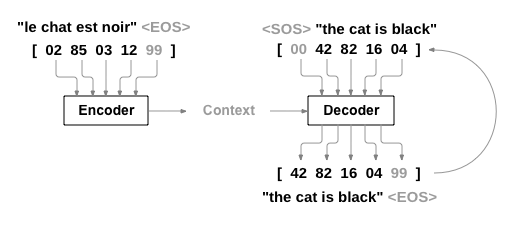
\includegraphics[width=0.5\linewidth,keepaspectratio]{seq1}
\end{center}     
\end{frame} 

%%%%%%%%%%%%%%%%%%%%%%%%%%%%%%%%%%%%%%%%%%%%%%%%%%%%%%%%%%%%%%%%%%%%%%%%%%%%%%%%%%
\begin{frame}[fragile]
\frametitle{ Loading data files}
\begin{itemize}
\item Data: A set of many thousands of English to French translation pairs.
\item Original Site: http://www.manythings.org/anki/fra-eng.zip
\item Download the data from https://download.pytorch.org/tutorial/data.zip and extract it to the current directory.
\item The file is a tab separated list of translation pairs:
\end{itemize}
\begin{lstlisting}    
I am cold.    J'ai froid.
\end{lstlisting}         
\end{frame} 

%%%%%%%%%%%%%%%%%%%%%%%%%%%%%%%%%%%%%%%%%%%%%%%%%%%%%%%%%%%%%%%%%%%%%%%%%%%%%%%%%%
\begin{frame}[fragile]
\frametitle{ Imports}
\begin{lstlisting}    
from __future__ import unicode_literals, print_function, division
from io import open
import unicodedata
import string
import re
import random

import torch
import torch.nn as nn
from torch import optim
import torch.nn.functional as F

device = torch.device("cuda" if torch.cuda.is_available() else "cpu")
\end{lstlisting}         
\end{frame} 
%%%%%%%%%%%%%%%%%%%%%%%%%%%%%%%%%%%%%%%%%%%%%%%%%%%%%%%%%%%%%%%%%%%%%%%%%%%%%%%%%%
\begin{frame}[fragile]
\frametitle{Processing}
\begin{itemize}
\item We will be representing each word in a language as a one-hot vector.
\item Will limit and trim the data to only use a few thousand words per language.
\item We'll need a unique index per word to use as the inputs and targets of the networks later, also.
\item To keep track of all this we will use a helper class called Lang which has word $\rightarrow$ index (word2index) and index $\rightarrow$ word (index2word) dictionaries, as well as a count of each word word2count to use to later replace rare words.
\end{itemize}
   
\end{frame} 

%%%%%%%%%%%%%%%%%%%%%%%%%%%%%%%%%%%%%%%%%%%%%%%%%%%%%%%%%%%%%%%%%%%%%%%%%%%%%%%%%%
\begin{frame}[fragile]
\frametitle{Processing}
\begin{lstlisting}    
SOS_token = 0
EOS_token = 1
class Lang:
    def __init__(self, name):
        self.name = name
        self.word2index = {}
        self.word2count = {}
        self.index2word = {0: "SOS", 1: "EOS"}
        self.n_words = 2  # Count SOS and EOS
    def addSentence(self, sentence):
        for word in sentence.split(' '):
            self.addWord(word)
    def addWord(self, word):
        if word not in self.word2index:
            self.word2index[word] = self.n_words
            self.word2count[word] = 1
            self.index2word[self.n_words] = word
            self.n_words += 1
        else:
            self.word2count[word] += 1
\end{lstlisting}   
   
\end{frame} 

%%%%%%%%%%%%%%%%%%%%%%%%%%%%%%%%%%%%%%%%%%%%%%%%%%%%%%%%%%%%%%%%%%%%%%%%%%%%%%%%%%
\begin{frame}[fragile]
\frametitle{ Language}
\begin{itemize}
\item As data has french, the input file is in Unicode
\item Just to simplify we will turn Unicode characters to ASCII, make everything lowercase, and trim most punctuation.
\end{itemize}
\begin{lstlisting}    
# Turn a Unicode string to plain ASCII, thanks to
# http://stackoverflow.com/a/518232/2809427
def unicodeToAscii(s):
    return ' '.join(c for c in unicodedata.normalize('NFD', s) if unicodedata.category(c) != 'Mn')

# Lowercase, trim, and remove non-letter characters
def normalizeString(s):
    s = unicodeToAscii(s.lower().strip())
    s = re.sub(r"([.!?])", r" \1", s)
    s = re.sub(r"[^a-zA-Z.!?]+", r" ", s)
    return s
\end{lstlisting}         
\end{frame} 

%%%%%%%%%%%%%%%%%%%%%%%%%%%%%%%%%%%%%%%%%%%%%%%%%%%%%%%%%%%%%%%%%%%%%%%%%%%%%%%%%%
\begin{frame}[fragile]
\frametitle{ Language}
\begin{itemize}
\item To read the data file we will split the file into lines, and then split lines into pairs. 
\item The files are all English $\rightarrow$ Other Language, so if we want to translate in reverse, flag is provided.
\end{itemize}
\begin{lstlisting}    
def readLangs(lang1, lang2, reverse=False):
    lines = open('data/%s-%s.txt' % (lang1, lang2), encoding='utf-8'). read().strip().split('\n')
    pairs = [[normalizeString(s) for s in l.split('\t')] for l in lines]
    if reverse:
        pairs = [list(reversed(p)) for p in pairs]
        input_lang = Lang(lang2)
        output_lang = Lang(lang1)
    else:
        input_lang = Lang(lang1)
        output_lang = Lang(lang2)

    return input_lang, output_lang, pairs
\end{lstlisting}         
\end{frame} 

%%%%%%%%%%%%%%%%%%%%%%%%%%%%%%%%%%%%%%%%%%%%%%%%%%%%%%%%%%%%%%%%%%%%%%%%%%%%%%%%%%
\begin{frame}[fragile]
\frametitle{ Language}
\begin{itemize}
\item To may a toy problem , we will use only relatively short and simple sentences. 
\item Will allow maximum length as 10 words (that includes ending punctuation) 
\end{itemize}
\begin{lstlisting}    
MAX_LENGTH = 10
eng_prefixes = (
    "i am ", "i m ",
    "he is", "he s ",
    "she is", "she s",
    "you are", "you re ",
    "we are", "we re ",
    "they are", "they re "
)
def filterPair(p):
    return len(p[0].split(' ')) < MAX_LENGTH and \
        len(p[1].split(' ')) < MAX_LENGTH and \
        p[1].startswith(eng_prefixes)
def filterPairs(pairs):
    return [pair for pair in pairs if filterPair(pair)]
\end{lstlisting}         
\end{frame} 

%%%%%%%%%%%%%%%%%%%%%%%%%%%%%%%%%%%%%%%%%%%%%%%%%%%%%%%%%%%%%%%%%%%%%%%%%%%%%%%%%%
\begin{frame}[fragile]
\frametitle{ Data Preprocessing}
The full process for preparing the data is:
\begin{itemize}
\item Read text file and split into lines, split lines into pairs
\item Normalize text, filter by length and content
\item Make word lists from sentences in pairs
\end{itemize}
      
\end{frame} 

%%%%%%%%%%%%%%%%%%%%%%%%%%%%%%%%%%%%%%%%%%%%%%%%%%%%%%%%%%%%%%%%%%%%%%%%%%%%%%%%%%
\begin{frame}[fragile]
\frametitle{ Data Preprocessing}
The full process for preparing the data is:
\begin{lstlisting}    
def prepareData(lang1, lang2, reverse=False):
    input_lang, output_lang, pairs = readLangs(lang1, lang2, reverse)
    print("Read %s sentence pairs" % len(pairs))
    pairs = filterPairs(pairs)
    print("Trimmed to %s sentence pairs" % len(pairs))
    print("Counting words...")
    for pair in pairs:
        input_lang.addSentence(pair[0])
        output_lang.addSentence(pair[1])
    print("Counted words:")
    print(input_lang.name, input_lang.n_words)
    print(output_lang.name, output_lang.n_words)
    return input_lang, output_lang, pairs
input_lang, output_lang, pairs = prepareData('eng', 'fra', True)
print(random.choice(pairs))
\end{lstlisting} 
      
\end{frame} 

%%%%%%%%%%%%%%%%%%%%%%%%%%%%%%%%%%%%%%%%%%%%%%%%%%%%%%%%%%%%%%%%%%%%%%%%%%%%%%%%%%
\begin{frame}[fragile]
\frametitle{ Data Preprocessing}
Output
\begin{lstlisting}    
>>>Reading lines...
Read 135842 sentence pairs
Trimmed to 10853 sentence pairs
Counting words...
Counted words:
fra 4489
eng 2925
['il est heroino dependant .', 'he is a heroin addict .']
\end{lstlisting} 
      
\end{frame} 

%%%%%%%%%%%%%%%%%%%%%%%%%%%%%%%%%%%%%%%%%%%%%%%%%%%%%%%%%%%%%%%%%%%%%%%%%%%%%%%%%%
\begin{frame}[fragile]
\frametitle{The Seq2Seq Model}

\begin{itemize}
\item Unlike sequence prediction with a single RNN, where every input corresponds to an output, 
\item the seq2seq model frees us from sequence length and order, 
\item which makes it ideal for translation between two languages, where number of words and order on both sides could vary.
\end{itemize}
      
\end{frame} 

%%%%%%%%%%%%%%%%%%%%%%%%%%%%%%%%%%%%%%%%%%%%%%%%%%%%%%%%%%%%%%%%%%%%%%%%%%%%%%%%%%
\begin{frame}[fragile]
\frametitle{The Encoder}

\begin{itemize}
\item The encoder of a seq2seq network is a RNN that outputs some value for every word from the input sentence.
\item For every input word the encoder outputs a vector and a hidden state, and uses the hidden state for the next input word.
\end{itemize}
\begin{center}
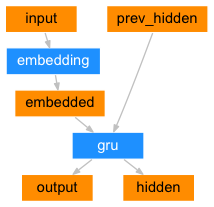
\includegraphics[width=0.5\linewidth,keepaspectratio]{seq2}
\end{center}           
\end{frame} 

%%%%%%%%%%%%%%%%%%%%%%%%%%%%%%%%%%%%%%%%%%%%%%%%%%%%%%%%%%%%%%%%%%%%%%%%%%%%%%%%%%
\begin{frame}[fragile]
\frametitle{The Encoder}
\begin{lstlisting}    
class EncoderRNN(nn.Module):
    def __init__(self, input_size, hidden_size):
        super(EncoderRNN, self).__init__()
        self.hidden_size = hidden_size

        self.embedding = nn.Embedding(input_size, hidden_size)
        self.gru = nn.GRU(hidden_size, hidden_size)

    def forward(self, input, hidden):
        embedded = self.embedding(input).view(1, 1, -1)
        output = embedded
        output, hidden = self.gru(output, hidden)
        return output, hidden

    def initHidden(self):
        return torch.zeros(1, 1, self.hidden_size, device=device)
\end{lstlisting} 
      
\end{frame} 

%%%%%%%%%%%%%%%%%%%%%%%%%%%%%%%%%%%%%%%%%%%%%%%%%%%%%%%%%%%%%%%%%%%%%%%%%%%%%%%%%%
\begin{frame}[fragile]
\frametitle{The Decoder}

\begin{itemize}
\item The decoder is another RNN that takes the encoder output vector(s) and outputs a sequence of words to create the translation
\item In the simplest seq2seq decoder we use only last output of the encoder. 
\item This last output is sometimes called the context vector as it encodes context from the entire sequence. 
\item This context vector is used as the initial hidden state of the decoder.
\end{itemize}
        
\end{frame} 


%%%%%%%%%%%%%%%%%%%%%%%%%%%%%%%%%%%%%%%%%%%%%%%%%%%%%%%%%%%%%%%%%%%%%%%%%%%%%%%%%%
\begin{frame}[fragile]
\frametitle{The Decoder}

\begin{itemize}
\item At every step of decoding, the decoder is given an input token and hidden state. 
\item The initial input token is the start-of-string <SOS> token, and the first hidden state is the context vector (the encoder's last hidden state)
\end{itemize}
\begin{center}
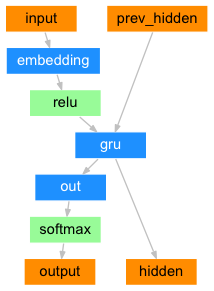
\includegraphics[width=0.5\linewidth,keepaspectratio]{seq3}
\end{center}           
\end{frame} 

%%%%%%%%%%%%%%%%%%%%%%%%%%%%%%%%%%%%%%%%%%%%%%%%%%%%%%%%%%%%%%%%%%%%%%%%%%%%%%%%%%
\begin{frame}[fragile]
\frametitle{The Decoder}
\begin{lstlisting}    
class DecoderRNN(nn.Module):
    def __init__(self, hidden_size, output_size):
        super(DecoderRNN, self).__init__()
        self.hidden_size = hidden_size

        self.embedding = nn.Embedding(output_size, hidden_size)
        self.gru = nn.GRU(hidden_size, hidden_size)
        self.out = nn.Linear(hidden_size, output_size)
        self.softmax = nn.LogSoftmax(dim=1)

    def forward(self, input, hidden):
        output = self.embedding(input).view(1, 1, -1)
        output = F.relu(output)
        output, hidden = self.gru(output, hidden)
        output = self.softmax(self.out(output[0]))
        return output, hidden

    def initHidden(self):
        return torch.zeros(1, 1, self.hidden_size, device=device)
 
\end{lstlisting} 
      
\end{frame} 

%%%%%%%%%%%%%%%%%%%%%%%%%%%%%%%%%%%%%%%%%%%%%%%%%%%%%%%%%%%%%%%%%%%%%%%%%%%%%%%%%%
\begin{frame}[fragile]
\frametitle{The Attention Decoder}

\begin{itemize}
\item If only the context vector is passed betweeen the encoder and decoder, that single vector carries the burden of encoding the entire sentence.
\item Attention allows the decoder network to ''focus'' on a different part of the encoder's outputs for every step of the decoder's own outputs.
\item First we calculate a set of attention weights. These will be multiplied by the encoder output vectors to create a weighted combination. 
\item The result (called attn\_applied in the code) should contain information about that specific part of the input sequence, and thus help the decoder choose the right output words.
\end{itemize}
        
\end{frame} 


%%%%%%%%%%%%%%%%%%%%%%%%%%%%%%%%%%%%%%%%%%%%%%%%%%%%%%%%%%%%%%%%%%%%%%%%%%%%%%%%%%
\begin{frame}[fragile]
\frametitle{The Attention Decoder}

Calculating the attention weights is done with another feed-forward layer attn, using the decoder's input and hidden state as inputs. 

\begin{center}
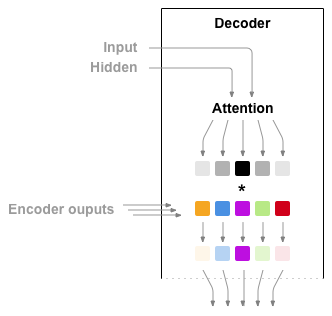
\includegraphics[width=0.5\linewidth,keepaspectratio]{seq4}
\end{center}           
\end{frame} 


%%%%%%%%%%%%%%%%%%%%%%%%%%%%%%%%%%%%%%%%%%%%%%%%%%%%%%%%%%%%%%%%%%%%%%%%%%%%%%%%%%
\begin{frame}[fragile]
\frametitle{The Attention Decoder}

\begin{itemize}
\item Because there are sentences of all sizes in the training data, to actually create and train this layer we have to choose a maximum sentence length (input length, for encoder outputs) that it can apply to. 
\item Sentences of the maximum length will use all the attention weights, while shorter sentences will only use the first few.
\end{itemize}
        
\end{frame} 

%%%%%%%%%%%%%%%%%%%%%%%%%%%%%%%%%%%%%%%%%%%%%%%%%%%%%%%%%%%%%%%%%%%%%%%%%%%%%%%%%%
\begin{frame}[fragile]
\frametitle{The Attention Decoder}
\begin{center}
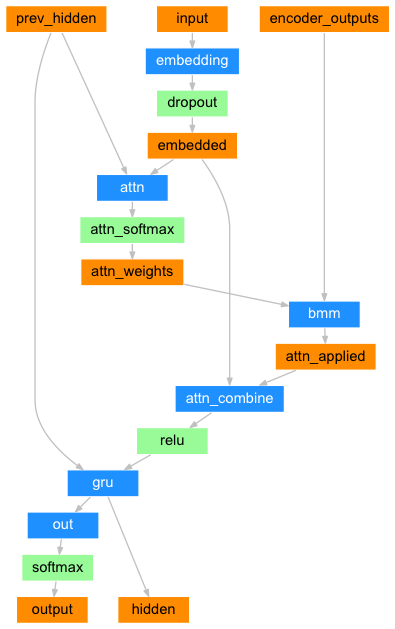
\includegraphics[width=0.4\linewidth,keepaspectratio]{seq5}
\end{center}           
\end{frame} 

%%%%%%%%%%%%%%%%%%%%%%%%%%%%%%%%%%%%%%%%%%%%%%%%%%%%%%%%%%%%%%%%%%%%%%%%%%%%%%%%%%
\begin{frame}[fragile]
\frametitle{The Attention Decoder}
\begin{lstlisting}    
class AttnDecoderRNN(nn.Module):
    def __init__(self, hidden_size, output_size, dropout_p=0.1, max_length=MAX_LENGTH):
        super(AttnDecoderRNN, self).__init__()
        self.hidden_size = hidden_size
        self.output_size = output_size
        self.dropout_p = dropout_p
        self.max_length = max_length

        self.embedding = nn.Embedding(self.output_size, self.hidden_size)
        self.attn = nn.Linear(self.hidden_size * 2, self.max_length)
        self.attn_combine = nn.Linear(self.hidden_size * 2, self.hidden_size)
        self.dropout = nn.Dropout(self.dropout_p)
        self.gru = nn.GRU(self.hidden_size, self.hidden_size)
        self.out = nn.Linear(self.hidden_size, self.output_size)
 \end{lstlisting} 
      
\end{frame} 
%%%%%%%%%%%%%%%%%%%%%%%%%%%%%%%%%%%%%%%%%%%%%%%%%%%%%%%%%%%%%%%%%%%%%%%%%%%%%%%%%%
\begin{frame}[fragile]
\frametitle{The Attention Decoder}
\begin{lstlisting}    
    def forward(self, input, hidden, encoder_outputs):
        embedded = self.embedding(input).view(1, 1, -1)
        embedded = self.dropout(embedded)

        attn_weights = F.softmax(
            self.attn(torch.cat((embedded[0], hidden[0]), 1)), dim=1)
        attn_applied = torch.bmm(attn_weights.unsqueeze(0),
                                 encoder_outputs.unsqueeze(0))

        output = torch.cat((embedded[0], attn_applied[0]), 1)
        output = self.attn_combine(output).unsqueeze(0)

        output = F.relu(output)
        output, hidden = self.gru(output, hidden)

        output = F.log_softmax(self.out(output[0]), dim=1)
        return output, hidden, attn_weights

    def initHidden(self):
        return torch.zeros(1, 1, self.hidden_size, device=device)
 \end{lstlisting} 
      
\end{frame} 

%%%%%%%%%%%%%%%%%%%%%%%%%%%%%%%%%%%%%%%%%%%%%%%%%%%%%%%%%%%%%%%%%%%%%%%%%%%%%%%%%%
\begin{frame}[fragile]
\frametitle{Preparing Training Data}

\begin{itemize}
\item To train, for each pair we will need an input tensor (indexes of the words in the input sentence) and target tensor (indexes of the words in the target sentence).
\item While creating these vectors we will append the EOS token to both sequences.
\end{itemize}
\begin{lstlisting}    
def indexesFromSentence(lang, sentence):
    return [lang.word2index[word] for word in sentence.split(' ')]
def tensorFromSentence(lang, sentence):
    indexes = indexesFromSentence(lang, sentence)
    indexes.append(EOS_token)
    return torch.tensor(indexes, dtype=torch.long, device=device).view(-1, 1)
def tensorsFromPair(pair):
    input_tensor = tensorFromSentence(input_lang, pair[0])
    target_tensor = tensorFromSentence(output_lang, pair[1])
    return (input_tensor, target_tensor)
 \end{lstlisting} 
              
\end{frame} 

%%%%%%%%%%%%%%%%%%%%%%%%%%%%%%%%%%%%%%%%%%%%%%%%%%%%%%%%%%%%%%%%%%%%%%%%%%%%%%%%%%
\begin{frame}[fragile]
\frametitle{Training the Model}

\begin{itemize}
\item To train we run the input sentence through the encoder, and keep track of every output and the latest hidden state. 
\item Then the decoder is given the $<SOS>$ token as its first input, and the last hidden state of the encoder as its first hidden state.
\end{itemize}
        
\end{frame} 

%%%%%%%%%%%%%%%%%%%%%%%%%%%%%%%%%%%%%%%%%%%%%%%%%%%%%%%%%%%%%%%%%%%%%%%%%%%%%%%%%%
\begin{frame}[fragile]
\frametitle{Training the Model}

\begin{itemize}
\item 'Teacher forcing' is the concept of using the real target outputs as each next input, instead of using the decoder's guess as the next input. 
\item Using teacher forcing causes it to converge faster but when the trained network is exploited, it may exhibit instability.
\item We can randomly choose to use teacher forcing or not with a simple if statement. Turn teacher\_forcing\_ratio up to use more of it.
\end{itemize}
        
\end{frame} 

%%%%%%%%%%%%%%%%%%%%%%%%%%%%%%%%%%%%%%%%%%%%%%%%%%%%%%%%%%%%%%%%%%%%%%%%%%%%%%%%%%
\begin{frame}[fragile]
\frametitle{Training the Model}
\begin{lstlisting}    
teacher_forcing_ratio = 0.5

def train(input_tensor, target_tensor, encoder, decoder, encoder_optimizer, decoder_optimizer, criterion, max_length=MAX_LENGTH):
    encoder_hidden = encoder.initHidden()

    encoder_optimizer.zero_grad()
    decoder_optimizer.zero_grad()

    input_length = input_tensor.size(0)
    target_length = target_tensor.size(0)

    encoder_outputs = torch.zeros(max_length, encoder.hidden_size, device=device)

 \end{lstlisting} 
              
\end{frame} 

%%%%%%%%%%%%%%%%%%%%%%%%%%%%%%%%%%%%%%%%%%%%%%%%%%%%%%%%%%%%%%%%%%%%%%%%%%%%%%%%%%
\begin{frame}[fragile]
\frametitle{Training the Model}
\begin{lstlisting}    
    loss = 0

    for ei in range(input_length):
        encoder_output, encoder_hidden = encoder(
            input_tensor[ei], encoder_hidden)
        encoder_outputs[ei] = encoder_output[0, 0]

    decoder_input = torch.tensor([[SOS_token]], device=device)

    decoder_hidden = encoder_hidden

	use_teacher_forcing = True if random.random() < teacher_forcing_ratio else False
 \end{lstlisting} 
              
\end{frame} 

%%%%%%%%%%%%%%%%%%%%%%%%%%%%%%%%%%%%%%%%%%%%%%%%%%%%%%%%%%%%%%%%%%%%%%%%%%%%%%%%%%
\begin{frame}[fragile]
\frametitle{Training the Model}
\begin{lstlisting}    
    if use_teacher_forcing:
        # Teacher forcing: Feed the target as the next input
        for di in range(target_length):
            decoder_output, decoder_hidden, decoder_attention = decoder(
                decoder_input, decoder_hidden, encoder_outputs)
            loss += criterion(decoder_output, target_tensor[di])
            decoder_input = target_tensor[di]  # Teacher forcing

\end{lstlisting} 
              
\end{frame} 

%%%%%%%%%%%%%%%%%%%%%%%%%%%%%%%%%%%%%%%%%%%%%%%%%%%%%%%%%%%%%%%%%%%%%%%%%%%%%%%%%%
\begin{frame}[fragile]
\frametitle{Training the Model}
\begin{lstlisting}    
    else:
        # Without teacher forcing: use its own predictions as the next input
        for di in range(target_length):
            decoder_output, decoder_hidden, decoder_attention = decoder(
                decoder_input, decoder_hidden, encoder_outputs)
            topv, topi = decoder_output.topk(1)
            decoder_input = topi.squeeze().detach()  # detach from history as input

            loss += criterion(decoder_output, target_tensor[di])
            if decoder_input.item() == EOS_token:
                break
\end{lstlisting} 
              
\end{frame} 


%%%%%%%%%%%%%%%%%%%%%%%%%%%%%%%%%%%%%%%%%%%%%%%%%%%%%%%%%%%%%%%%%%%%%%%%%%%%%%%%%%
\begin{frame}[fragile]
\frametitle{Training the Model}
\begin{lstlisting}    
    loss.backward()

    encoder_optimizer.step()
    decoder_optimizer.step()

    return loss.item() / target_length
\end{lstlisting} 
              
\end{frame} 

%%%%%%%%%%%%%%%%%%%%%%%%%%%%%%%%%%%%%%%%%%%%%%%%%%%%%%%%%%%%%%%%%%%%%%%%%%%%%%%%%%
\begin{frame}[fragile]
\frametitle{Helper Utility}
\begin{lstlisting}    
import time
import math


def asMinutes(s):
    m = math.floor(s / 60)
    s -= m * 60
    return '%dm %ds' % (m, s)


def timeSince(since, percent):
    now = time.time()
    s = now - since
    es = s / (percent)
    rs = es - s
    return '%s (- %s)' % (asMinutes(s), asMinutes(rs))
\end{lstlisting} 
              
\end{frame} 

%%%%%%%%%%%%%%%%%%%%%%%%%%%%%%%%%%%%%%%%%%%%%%%%%%%%%%%%%%%%%%%%%%%%%%%%%%%%%%%%%%
\begin{frame}[fragile]
\frametitle{Training the Model}
The whole training process looks like this:
\begin{itemize}
\item Start a timer
\item Initialize optimizers and criterion
\item Create set of training pairs
\item Start empty losses array for plotting
\end{itemize}
Then we call train many times and occasionally print the progress (\% of examples, time so far, estimated time) and average loss.              
\end{frame} 

%%%%%%%%%%%%%%%%%%%%%%%%%%%%%%%%%%%%%%%%%%%%%%%%%%%%%%%%%%%%%%%%%%%%%%%%%%%%%%%%%%
\begin{frame}[fragile]
\frametitle{Helper Utility}
\begin{lstlisting}    
def trainIters(encoder, decoder, n_iters, print_every=1000, plot_every=100, learning_rate=0.01):
    start = time.time()
    plot_losses = []
    print_loss_total = 0  # Reset every print_every
    plot_loss_total = 0  # Reset every plot_every

    encoder_optimizer = optim.SGD(encoder.parameters(), lr=learning_rate)
    decoder_optimizer = optim.SGD(decoder.parameters(), lr=learning_rate)
    training_pairs = [tensorsFromPair(random.choice(pairs))
                      for i in range(n_iters)]
    criterion = nn.NLLLoss()
\end{lstlisting} 
              
\end{frame} 

%%%%%%%%%%%%%%%%%%%%%%%%%%%%%%%%%%%%%%%%%%%%%%%%%%%%%%%%%%%%%%%%%%%%%%%%%%%%%%%%%%
\begin{frame}[fragile]
\frametitle{Helper Utility}
\begin{lstlisting}    
    for iter in range(1, n_iters + 1):
        training_pair = training_pairs[iter - 1]
        input_tensor = training_pair[0]
        target_tensor = training_pair[1]

        loss = train(input_tensor, target_tensor, encoder,
                     decoder, encoder_optimizer, decoder_optimizer, criterion)
        print_loss_total += loss
        plot_loss_total += loss

        if iter % print_every == 0:
            print_loss_avg = print_loss_total / print_every
            print_loss_total = 0
            print('%s (%d %d%%) %.4f' % (timeSince(start, iter / n_iters),
                                         iter, iter / n_iters * 100, print_loss_avg))

        if iter % plot_every == 0:
            plot_loss_avg = plot_loss_total / plot_every
            plot_losses.append(plot_loss_avg)
            plot_loss_total = 0

    showPlot(plot_losses)
\end{lstlisting} 
              
\end{frame} 

%%%%%%%%%%%%%%%%%%%%%%%%%%%%%%%%%%%%%%%%%%%%%%%%%%%%%%%%%%%%%%%%%%%%%%%%%%%%%%%%%%
\begin{frame}[fragile]
\frametitle{Plotting results}
Plotting is done with matplotlib, using the array of loss values plot\_losses saved while training.
\begin{lstlisting}    
import matplotlib.pyplot as plt
plt.switch_backend('agg')
import matplotlib.ticker as ticker
import numpy as np


def showPlot(points):
    plt.figure()
    fig, ax = plt.subplots()
    # this locator puts ticks at regular intervals
    loc = ticker.MultipleLocator(base=0.2)
    ax.yaxis.set_major_locator(loc)
    plt.plot(points)
\end{lstlisting} 
              
\end{frame} 

%%%%%%%%%%%%%%%%%%%%%%%%%%%%%%%%%%%%%%%%%%%%%%%%%%%%%%%%%%%%%%%%%%%%%%%%%%%%%%%%%%
\begin{frame}[fragile]
\frametitle{Evaluation}
\begin{itemize}
\item Evaluation is mostly the same as training, but there are no targets so we simply feed the decoder's predictions back to itself for each step. 
\item Every time it predicts a word we add it to the output string, and if it predicts the EOS token we stop there. 
\item We also store the decoder's attention outputs for display later.
\end{itemize}

\end{frame} 

%%%%%%%%%%%%%%%%%%%%%%%%%%%%%%%%%%%%%%%%%%%%%%%%%%%%%%%%%%%%%%%%%%%%%%%%%%%%%%%%%%
\begin{frame}[fragile]
\frametitle{Evaluation}
\begin{lstlisting}    
def evaluate(encoder, decoder, sentence, max_length=MAX_LENGTH):
    with torch.no_grad():
        input_tensor = tensorFromSentence(input_lang, sentence)
        input_length = input_tensor.size()[0]
        encoder_hidden = encoder.initHidden()

        encoder_outputs = torch.zeros(max_length, encoder.hidden_size, device=device)

        for ei in range(input_length):
            encoder_output, encoder_hidden = encoder(input_tensor[ei],
                                                     encoder_hidden)
            encoder_outputs[ei] += encoder_output[0, 0]

        decoder_input = torch.tensor([[SOS_token]], device=device)  # SOS

        decoder_hidden = encoder_hidden

        decoded_words = []
        decoder_attentions = torch.zeros(max_length, max_length)
\end{lstlisting} 
              
\end{frame} 


%%%%%%%%%%%%%%%%%%%%%%%%%%%%%%%%%%%%%%%%%%%%%%%%%%%%%%%%%%%%%%%%%%%%%%%%%%%%%%%%%%
\begin{frame}[fragile]
\frametitle{Evaluation}
\begin{lstlisting}    
        for di in range(max_length):
            decoder_output, decoder_hidden, decoder_attention = decoder(
                decoder_input, decoder_hidden, encoder_outputs)
            decoder_attentions[di] = decoder_attention.data
            topv, topi = decoder_output.data.topk(1)
            if topi.item() == EOS_token:
                decoded_words.append('<EOS>')
                break
            else:
                decoded_words.append(output_lang.index2word[topi.item()])

            decoder_input = topi.squeeze().detach()

        return decoded_words, decoder_attentions[:di + 1]
\end{lstlisting} 
              
\end{frame} 


%%%%%%%%%%%%%%%%%%%%%%%%%%%%%%%%%%%%%%%%%%%%%%%%%%%%%%%%%%%%%%%%%%%%%%%%%%%%%%%%%%
\begin{frame}[fragile]
\frametitle{Training and Evaluating}
\begin{itemize}
\item Remember that the input sentences were heavily filtered. 
\item For this small dataset we can use relatively small networks of 256 hidden nodes and a single GRU layer.
\item After about 40 minutes on a MacBook CPU we’ll get some reasonable results.
\end{itemize}
\begin{lstlisting}    
hidden_size = 256
encoder1 = EncoderRNN(input_lang.n_words, hidden_size).to(device)
attn_decoder1 = AttnDecoderRNN(hidden_size, output_lang.n_words, dropout_p=0.1).to(device)

trainIters(encoder1, attn_decoder1, 75000, print_every=5000)

evaluateRandomly(encoder1, attn_decoder1)
\end{lstlisting}
              
\end{frame} 
